\documentclass[10pt,a4paper]{article}
\usepackage[utf8]{inputenc}
\usepackage{amsmath}
\usepackage{amsfonts}
\usepackage{amssymb}
\usepackage{graphicx}
\graphicspath{{img/}}
\author{150016853}
\title{Player Guide - MorphZone}
\begin{document}

\section{Menu}

Be sure to select a map and floor mode. The changes you've made will be shown behind you.

\begin{figure}[!h]
\centering
  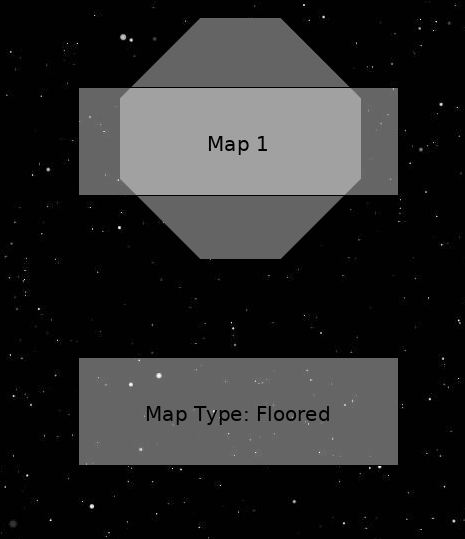
\includegraphics[scale=0.5]{menu_options.png}
  \caption{Map options.}
  \label{fig:boat1}
\end{figure}

\section{Player Controls}

\subsection{Player 1}

\subsubsection*{All Modes}

\makebox[1cm]{C} \makebox[0.5cm]{-} Switch To Boosting Mode
\\\makebox[1cm]{V} \makebox[0.5cm]{-} Switch To Tether Mode
\\\makebox[1cm]{B} \makebox[0.5cm]{-} Switch To Dropper Mode

\subsubsection*{Boosting Mode}

\makebox[1cm]{W} \makebox[0.5cm]{-} Boost
\\\makebox[1cm]{A} \makebox[0.5cm]{-} Rotate Left
\\\makebox[1cm]{D} \makebox[0.5cm]{-} Rotate Right
\\\makebox[1cm]{Space} \makebox[0.5cm]{-} Fire

\subsubsection*{Tether Mode}

\makebox[1cm]{A} \makebox[0.5cm]{-} Tether Left
\\\makebox[1cm]{D} \makebox[0.5cm]{-} Tether Right

\subsubsection*{Dropper Mode}

No Additional Controls

\subsection{Player 2}


\subsubsection{All Modes}

\makebox[1cm]{P} \makebox[0.5cm]{-} Switch To Boosting Mode
\\\makebox[1cm]{[} \makebox[0.5cm]{-} Switch To Tether Mode
\\\makebox[1cm]{]} \makebox[0.5cm]{-} Switch To Dropper Mode

\subsubsection*{Boosting Mode}

\makebox[4cm]{Up Arrow/Numpad 8} \makebox[0.5cm]{-} Boost
\\\makebox[4cm]{Left Arrow/Numpad 4} \makebox[0.5cm]{-} Rotate Left
\\\makebox[4cm]{Right Arrow/Numpad 6} \makebox[0.5cm]{-} Rotate Right
\\\makebox[4cm]{Space} \makebox[0.5cm]{-} Fire

\subsubsection*{Tether Mode}

\makebox[4cm]{Left Arrow/Numpad 4} \makebox[0.5cm]{-} Tether Left
\\\makebox[4cm]{Right Arrow/Numpad 6} \makebox[0.5cm]{-} Tether Right

\subsubsection*{Dropper Mode}

No Additional Controls

\section{Play Guide}

Shoot at your opponent when in boosting mode to knock them back into walls. When they hit a wall fast enough they take damage. If you can knock them back into a set of map lasers they will get destroyed immediately. When they die, you win.

Pick up power ups to get health and replace your current weapon with a new weapon.

\begin{figure}[!h]
\centering
  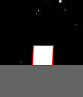
\includegraphics{health_powerup.png}
  \caption{Health Powerup.}
  \label{fig:boat1}
\end{figure}

\begin{figure}[!h]
\centering
  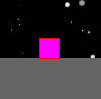
\includegraphics{weapon_powerup.png}
  \caption{Weapon Powerup.}
  \label{fig:boat1}
\end{figure}

Sometimes it helps to be on top of your opponent in terms of movement so you can use other modes to make things harder for your opponent, whether it's escaping them or catching them off guard.

When in boosting mode you can fly around and fire, but turning corners can be hard when you're that fast.

\begin{figure}[!h]
\centering
  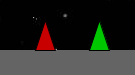
\includegraphics{boost_mode.png}
  \caption{Player 1 (Left) and Player 2 (Right) in boost mode.}
  \label{fig:boat1}
\end{figure}

Tether mode allows you to attach yourself to nearby objects (though not other players!) to turn corners very quickly whilst keeping speed. Two outlines highlight the range in which you can tether to objects. Be wary though, it can be difficult, especially if you're not keeping track of your orientation. Though not to worry, you take half damage in this form from collisions.

\begin{figure}[!h]
\centering
  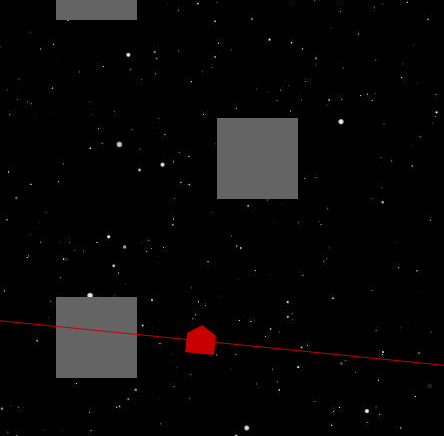
\includegraphics[width=\linewidth]{player_1_ready_tether.png}
  \caption{Player 1 ready to tether to the left in tether mode.}
  \label{fig:boat1}
\end{figure}

\begin{figure}[!h]
\centering
  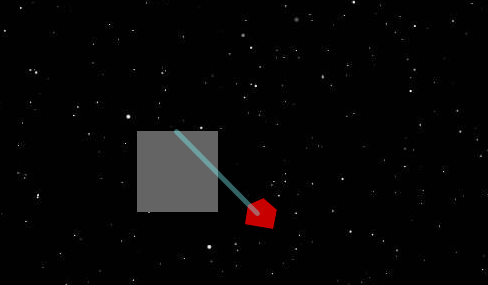
\includegraphics[scale = 0.5]{player_1_tethered.png}
  \caption{Player 1 tethered to an object.}
  \label{fig:boat1}
\end{figure}

When in dropper mode get a brief moment of respite where your character will pause, allowing you to stop all momentum. However you will be immediately propelled downwards, so watch out, it may cause you to die if you're not careful. You will also be vulnerable to enemy damage when stopped, so watch out. You can use this to propel yourself into tethers as well, getting lots of speed and allowing quick movement across the map.

\begin{figure}[!h]
\centering
  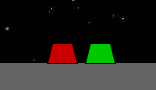
\includegraphics{dropper_mode.png}
  \caption{Player 1 (left) and Player 2 (right) in dropper mode.}
  \label{fig:boat1}
\end{figure}

Be sure to watch out for destroyer beams. These will eliminate you the moment you touch them.

\begin{figure}[!h]
\centering
  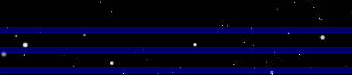
\includegraphics{destroyer_beams.png}
  \caption{Destroyer Beams.}
  \label{fig:boat1}
\end{figure}

\section{Advanced Tactics}

When transitioning between modes note how your orientation is preserved. If changing from any mode to your boost mode you will be pointing in the direction you were travelling, allowing you to keep your momentum! If you transition to tether mode from booster mode your orientation will point the same direction as travel, allowing you to tether in that direction. If you transition from dropper mode to tether mode you will be pointing straight up, allowing you to tether left or right with ease.

If you want to prevent another player from getting a pickup, you can shoot powerups and they will fly off into the distance, maybe giving you an advantage!


\end{document}